%%%
% LaTeX PREAMBLE
%%%

\documentclass[aspectratio=169]{beamer}

\mode<presentation>
{
  \usetheme{IMI} 
  \setbeamercovered{transparent} 
}

\usepackage{booktabs}
\usepackage[ngerman]{babel}
\usepackage{times}
\usepackage[T1]{fontenc}
\usepackage{tikz}
\usetikzlibrary{positioning}

\usepackage[
    backend=biber,
    style=authoryear,
    doi=false,
    isbn=false,
    url=false,
    eprint=false
]{biblatex}

\addbibresource{seminar_folien.bib}

%%%
% TITLE INFORMATION
%%%

\title[Automatisierte Entscheidungsunterstützung in der Medizin]
{Automatisierte Entscheidungsunterstützung in der Medizin}


\author{
  David Dietrich
  \\
  Mohammad Waheed Abdulbaki Shurbaji
  \\
  Sami Abou Alzahab
\\
}

\date{\today}

\institute {
  Institut für med. Informatik\\
  Universität zu Lübeck
}


%%%
% PRESENTATION FRAMES / SLIDES
%%%
\begin{document}

\begin{frame}
  \titlepage
\end{frame}

\begin{frame}{Inhaltsverzeichnis}
  \small
  \tableofcontents
\end{frame}


\section{Ist vollständige Erklärbarkeit überhaupt möglich?}

\begin{frame}{Eingangsfrage}
  \begin{center}
      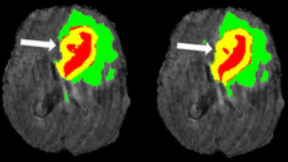
\includegraphics[width=0.5\textwidth]{images/image_01}
  \end{center}
 Ein Radiologe und ein KI-Modell erkennen
denselben Hirntumor.
\newline
Warum erwarten wir beim KI-Modell eine
vollständige Erklärung, beim Arzt aber nicht? \parencite{kemptRelativeExplainabilityDouble2022}
 \vfill
%   \hfill
  {\tiny Bild-Quelle: \fullcite{liLargeKernelAttention3D2023}}
\end{frame}

\begin{frame}{Transparenzproblem moderner KI}
 Neuronale Netze können als stark komprimierte Repräsentationen von Wissen betrachtet werden.
 \vspace{0.3cm}
 \begin{center}
\begin{tikzpicture}[
    node distance=0.5cm,
    box/.style={
        draw,
        rounded corners,
        align=center,
        minimum width=2.5cm,
        minimum height=0.8cm
    },
    arrow/.style={
        ->,
        thick
    }
]

\node[box] (data) {Trainingsdaten};
\node[box, right=of data] (training) {Training};
\node[box, right=of training] (params) {komprimiertes Wissen};
\node[box, right=of params] (decision) {Entscheidung};

\draw[arrow] (data) -- (training);
\draw[arrow] (training) -- (params);
\draw[arrow] (params) -- (decision);

\end{tikzpicture}
\end{center}
\vspace{0.3cm}
 Der Ursprung einzelner Entscheidungen ist
nicht mehr direkt nachvollziehbar.

 \vfill
%   \hfill
  {\tiny Technische Grundlage: \fullcite{wangUnderstandingDeepRepresentation2025}}
\end{frame}

\begin{frame}{Grenzen der Erklärbarkeit}
 Selbst moderne Explainable-AI-Verfahren
liefern häufig nur Hinweise.
\vspace{0.2cm}
\begin{itemize}
 \item Saliency Maps zeigen relevante Bildbereiche
 \item Unsicherheiten können visualisiert werden
 \item Der eigentliche Entscheidungsprozess bleibt
  jedoch oft verborgen
\end{itemize}
\vspace{0.2cm}
\rightarrow \vspace{0.1cm} Erklären wir die Ursache einer Entscheidung
  oder lediglich ihre nachträgliche Begründung? \parencite{rudinStopExplainingBlack2019}
\end{frame}

\begin{frame}{Gilt das nicht auch für Menschen?}
Menschen treffen viele Entscheidungen intuitiv.
\vspace{0.2cm}
\begin{itemize}
\item Gesichter erkennen
\item Sprache verwenden
\item Medizinische Diagnosen stellen
\end{itemize}
\vspace{0.2cm}
Das Ergebnis kann begründet werden,
der tatsächliche neuronale Prozess aber nicht. \parencite{nisbettTellingMoreWe1977}
\newline
\vspace{0.5cm}
\begin{center}
\textbf{Müssten wir nach derselben Logik nicht auch das menschliche Gehirn vollständig erklären können?}
\end{center}

\end{frame}

\begin{frame}{Fazit}
Vollständige Erklärbarkeit komplexer KI-Systeme
erscheint derzeit kaum erreichbar.\newline\newline
Entscheidend könnte daher weniger die vollständige
Nachvollziehbarkeit jedes Entscheidungsschritts
sein, sondern die Frage:\newline\newline
Ist das System zuverlässig genug und kommuniziert
es seine Unsicherheiten ausreichend, um
verantwortungsvolle Entscheidungen zu unterstützen?
 \vfill
%   \hfill
  {\tiny Quelle: \fullcite{kemptRelativeExplainabilityDouble2022}}
\end{frame}

\section{Fairness und Bias in der künstlichen Intelligenz}


% ==============================================================================
% FOLIE 3: BIAS TYPEN
% ==============================================================================
\begin{frame}[shrink]{Bias Typen}
    \small
    \renewcommand{\arraystretch}{1.5}
    \begin{center}
        \begin{tabular}{|p{0.24\textwidth}|p{0.35\textwidth}|p{0.35\textwidth}|}
            \hline
            \textbf{Bias-Typ} & \textbf{Beschreibung} & \textbf{Beispiele} \\
            \hline
            \textbf{Confirmation Bias} & Tritt auf, wenn ein KI-System verwendet wird, um bereits bestehende Vorurteile oder Überzeugungen seiner Entwickler oder Nutzer zu bestätigen. & Ein KI-System, das den Erfolg von Bewerbern auf der Grundlage von Vorurteilen des Personalmanagers vorhersagt. \\
            \hline
            \textbf{Measurement Bias} & Entsteht, wenn die Datenerfassung oder -messung bestimmte Gruppen systematisch über- oder unterrepräsentiert. & Eine Umfrage, die mehr Antworten von Stadtbewohnern sammelt, was zu einer Unterrepräsentation ländlicher Meinungen führt. \\
            \hline
            \textbf{Interaction Bias} & Tritt auf, wenn ein KI-System auf voreingenommene Weise mit Menschen interagiert, was zu einer unfairen Behandlung führt. & Ein Chatbot, der auf Männer und Frauen unterschiedlich reagiert, was zu einer verzerrten Kommunikation führt. \\
            \hline
        \end{tabular}
    \end{center}
    
    \vspace{0.2cm}
    \tiny \textit{Quelle: Fairness and Bias in Artificial Intelligence: A Brief Survey of Sources, Impacts, and Mitigation Strategies (Emilio Ferrara)}
\end{frame}


% ==============================================================================
% FOLIE 5: ZUVERLÄSSIG TROTZ KLARER VERZERRUNG?
% ==============================================================================
\begin{frame}{Zuverlässig trotz klarer Verzerrung?}
    \begin{itemize}
        \item Inwiefern wird eine ärztliche Entscheidung von einer KI beeinflusst?
        \item Hohe Genauigkeit allein garantiert keine Vertrauenswürdigkeit: (vgl. Studie zur \textit{Mobile App for diagnosis and management of pigmented skin cancer})
        \begin{itemize}
            \item Ein blindes Vertrauen in die KI-Entscheidungen hätte zu unnötigen Biopsien und Operationen geführt.
            \item Reine Diagnosemetriken sind nicht ausreichend; die klinische Erfahrung und Urteilskraft bleiben unverzichtbar.
        \end{itemize}
    \end{itemize}
    
    \vspace*{\fill}
    \tiny \textit{Quelle: Menzies S, Sinz C, Menzies M et al. \textbf{Comparison of humans versus mobile phone-powered artificial intelligence for the diagnosis and management of pigmented skin cancer in secondary care: a multicentre, prospective, diagnostic, clinical trial} The Lancet Digital Health, 5, e679-e691}
\end{frame}

% ==============================================================================
% FOLIE 6: INDIVIDUELLE UND GESELLSCHAFTLICHE AUSWIRKUNGEN
% ==============================================================================
\begin{frame}[shrink]{Individuelle und Gesellschaftliche Auswirkungen}
    \begin{columns}[T]
        \begin{column}{0.48\textwidth}
            \textbf{Individuelle Ebene}
            \begin{itemize}
                \item \textbf{Wandel des Arbeitsalltags:} KI als Assistenz ("Augmentation"), Wegfall von Routinen. \\
                \tiny \textit{(Quelle: BCG, 2023 – "AI Will Reshape More Jobs Than It Replaces")} \small
                \item \textbf{Hyper-Personalisierung:} Maßgeschneiderte Behandlungen (Medizin) und Lernwege (Bildung). \\
                \tiny \textit{(Quelle: The European Wergeland Centre, 2023)} \small
                \item \textbf{Autonomieverlust \& " Skill-Fading ":} Soziale Entfremdung und das Verlernen eigener Fähigkeiten. \\
                \tiny \textit{(Quelle: Chu et al., 2020 – PMC7605294)} \small
            \end{itemize}
        \end{column}
        
        \begin{column}{0.48\textwidth}
            \textbf{Gesellschaftliche Ebene}
            \begin{itemize}
                \item \textbf{Wirtschaftliche Ungleichheit:} Massive Gewinnkonzentration bei wenigen Tech-Akteuren. \\
                \tiny \textit{(Quelle: Fraunhofer IAO, 2021)} \small
                \item \textbf{Skalierung von Bias:} Automatisierte, massenhafte Reproduktion historischer Diskriminierung. \\
                \tiny \textit{(Quelle: Chu et al., 2020)} \small
                \item \textbf{Systemische Vulnerabilität:} Kontrollverlust und unvorhersehbare Kettenreaktionen durch "Black-Box"-Systeme. \\
                \tiny \textit{(Quelle: Chu et al., 2020)} \small
            \end{itemize}
        \end{column}
    \end{columns}
\end{frame}


% ==============================================================================
% FOLIE 7: GRENZEN DER TRANSPARENZ & VERANTWORTUNG
% ==============================================================================
\begin{frame}{Grenzen der Transparenz}
    \begin{itemize}
        \item \textbf{Transparenz $\neq$ Verantwortlichkeit:} Einblick in Daten und Algorithmen garantiert in der klinischen Anwendung keine automatische Haftung oder Verantwortung.
        \item \textbf{Ethisch-epistemische Hürden:} Selbst vollständig offengelegte Systeme werfen weiterhin grundlegende ethische Fragen bezüglich fehlerhafter Entscheidungen auf.
        \item \textbf{Regulatorische Realität:} Gesetzliche Vorgaben wie die DSGVO fordern primär allgemeine Systemtransparenz, bieten jedoch kein klares rechtliches „Recht auf Erklärung“ im Schadensfall.
    \end{itemize}
    
    \vspace*{\fill}
    \tiny \textit{Quellen: de Laat (2018); Herzog (2019, 2021); Wachter et al. (2017) -- Vgl. Stellungnahme der ZEKO BÄK (2021)}
\end{frame}

% ==============================================================================
% FOLIE 8: DAS PATIENTEN-DILEMMA
% ==============================================================================
\begin{frame}{Das Patienten-Dilemma}
    \begin{itemize}
        \item Würden Sie eine Klinik wählen, die sofortige Termine ohne Wartezeit bietet, aber zu 100\,\% von KI in Diagnostik und Therapie gesteuert wird?
        \item \textbf{Oder} bevorzugen Sie eine traditionelle Praxis mit langen Wartezeiten und 0\,\% KI-Unterstützung?
    \end{itemize}
\end{frame}


\section{KI als neuer Akteur im Sprechzimmer }

\begin{frame}{}

    \vspace{0.8cm}
    \begin{center}
        \textbf{\Large In der Theorie behalten wir Menschen die Kontrolle.} \\
        \vspace{0.4cm}
        \textbf{\Large Aber was passiert psychologisch mit uns, wenn die Maschine scheinbar alles besser weiß?}
    \end{center}
\end{frame}




\begin{frame}{Ist KI wirklich nur das nächste Ultraschallgerät?}
    \textit{,,Die Integration von KI in die Medizin verändert die Ärzt:in-Patient:in-Beziehung und die Rolle der Ärzt:innen grundlegend.''} \parencite{roche2025}
    
    \vspace{0.4cm}
    \textbf{Im Gegensatz zu klassischen Werkzeugen (z.\,B. Ultraschall):}
    \begin{itemize}
        \item KI liefert automatisierte Handlungs- und Entscheidungsempfehlungen.
        \item Die Technologie greift aktiv in soziale und psychologische Dynamiken ein.
    \end{itemize}

    \vfill
    {\tiny Quelle: \fullcite{roche2025}}
\end{frame}

\begin{frame}{Deskilling und der ,,Google-Maps-Effekt''}
    \textit{,,KI in der Diagnostik führt zu Kompetenzverlust bei Ärzten.''} \parencite{datenschutzticker2025}
    
    \vspace{0.4cm}
    \textbf{Das psychologische Problem:}
    \begin{itemize}
        \item Übermäßige Abhängigkeit von Systemen führt zur ,,leisen Erosion'' ärztlicher Kernfähigkeiten.
        \item Visuelle Suchgewohnheiten und eigene Mustererkennung stumpfen ab (Beispiel: Koloskopie-Studie).
    \end{itemize}

    \vfill
    {\tiny Quelle: \fullcite{datenschutzticker2025}}
\end{frame}

\begin{frame}{Die Koloskopie-Studie}
    \textbf{Studiendesign}
    \begin{itemize}
        \item 19 erfahrene Endoskopiker aus 4 Zentren.
        \item 1.443 Koloskopien analysiert (an Tagen \textit{ohne} KI, nach einer Eingewöhnungsphase an das System).
    \end{itemize}

    \vspace{0.4cm}
    \textbf{Kernergebnisse }
    \begin{itemize}
        \item \textbf{Signifikanter Abfall:} Ohne KI sank die ärztliche Erkennungsrate um 6 Prozent (von \textbf{28,4\,\%} auf \textbf{22,4\,\%}).
        \item \textbf{Der Maskierungseffekt:} Mit eingeschalteter KI stieg die ADR auf \textbf{25,3\,\%} -- der eigene Kompetenzverlust fiel im Alltag dadurch gar nicht auf.
    \end{itemize}

    \vspace{0.4cm}
    \textbf{Die Ursache}
    \begin{itemize}
        \item Die visuelle Mustererkennung der Ärzte stumpft durch die Technik-Abhängigkeit ab (,,Google-Maps-Effekt'').
    \end{itemize}

    \vfill
    {\tiny Quelle: \fullcite{datenschutzticker2025}}
\end{frame}

\begin{frame}{Von der Dyade zur multiplen Struktur}
    \textit{,,Lange Zeit war die medizinische Entscheidungsfindung eine Dyade. [...] Mit der Integration von KI in die Entscheidungsfindung stellt sich die Frage, ob diese Zweierbeziehung weiterhin bestehen bleibt oder ob sich der Prozess zu einer multiplen Entscheidungsstruktur weiterentwickelt.''} \parencite{roche2025}
    
    \vspace{0.4cm}
    \textbf{Die neue Realität:}
    \begin{center}
        Patient:in + Ärzt:in + Patienten-KI (z.\,B. ChatGPT) + Klinische KI
    \end{center}

    \vfill
    {\tiny Quelle: \fullcite{roche2025}}
\end{frame}


\begin{frame}{Fazit: Augmentation statt Automatisierung}
    \textit{,,Die Zukunft der medizinischen Entscheidungsfindung liegt nicht in der Frage, ob KI Entscheidungen trifft, sondern darin, wie wir Ärzt:innen, Patient:innen und KI gemeinsam zu besseren Entscheidungen kommen.''} \parencite{roche2025}
    
    \vspace{0.4cm}
    \begin{itemize}
        \item Mensch und Maschine müssen als Team funktionieren (\textit{Human-in-the-Loop}).
    \end{itemize}

    \vfill
    {\tiny Quelle: \fullcite{roche2025}}
\end{frame}



\section{Ausblick und Diskussion}
\begin{frame}{Die alles entscheidende Frage}

    \vspace{0.6cm}
    \begin{center}
        \textbf{\Large Soll die KI die endgültige Entscheidung treffen?} \\
        \vspace{0.4cm}
        \textbf{\Large Und wer trägt am Ende dafür die Verantwortung?}
    \end{center}
\end{frame}



\end{document}
